\section{Derivation of Navier-Stokes equation}
The goal of this section is to find an equation, which describes the spatio-temporal evolution of the velocity field $\vec{u}(\vec{r},t)$. This is the Navier-Stokes equation, which is the most fundamental equation in Fluid Dynamics.
\begin{figure}[!h]
    \centering
    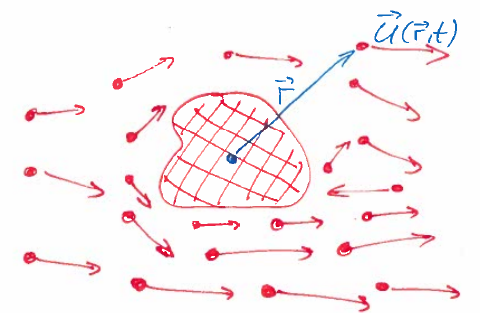
\includegraphics[width=.4\textwidth]{week2/velocity-field}
    \caption{Velocity field around an object.}
    \label{fig:velocity-field}
\end{figure}

We want to describe the motion of a fluid particle. We start with Newton's second law of Classical Mechanics
\begin{equation}
\vec{F} = \diff{}{t}\left(m\vec{u}\right).
\end{equation}
The equation states that the forces acting on the particle equals its change (the time derivative) of momentum (the parenthesis).
\begin{framed}
\textbf{Remark:} in Fluid Dynamics we look not only at one fluid particle, but at all fluid particles.
\end{framed}
\begin{equation}
\diff{}{t}\left(m\vec{u}\right) = \diff{m}{t}\vec{u}+m\diff{\vec{u}}{t}=\rho\Delta V\diff{\vec{u}}{t}.
\end{equation}
The mass of a fluid particle is constant and does not change over time, hence the time derivative term is zero. We also used the relation
\begin{equation}
m=\rho\Delta V.
\end{equation}
Given the field description $\vec{u}=\vec{u}(\vec{r},t)$, we have to be a little careful with $\diff{\vec{u}}{t}$. The following is wrong:
\begin{equation}
\diff{\vec{u}}{t} = \diff{\vec{u}(\vec{r},t)}{t} = \lim_{\Delta t \rightarrow 0} \frac{\vec{u}(\vec{r},t+\Delta t) - \vec{u}(\vec{r},t)}{\Delta t}
\end{equation}
See the example in \fref{fig:fluid-particles}.

\begin{figure}[!h]
    \centering
    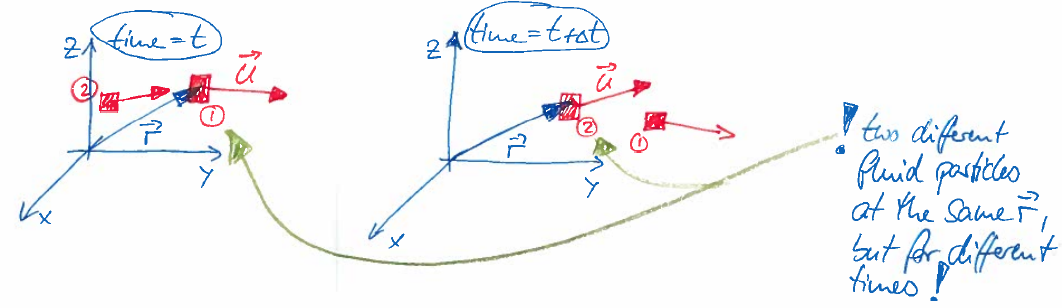
\includegraphics[width=.9\textwidth]{week2/fluid-particles}
    \caption{Two fluid particles can have the same coordinate vector $\vec{r}$ but for different times.}
    \label{fig:fluid-particles}
\end{figure}
The correct approach is to follow one fluid particle on its pathline (trajectory) $\vec{r}=\vec{r}(\vec{r}_0,t_0;t)$. See \fref{fig:fluid-particle}.
\begin{figure}[!h]
    \centering
    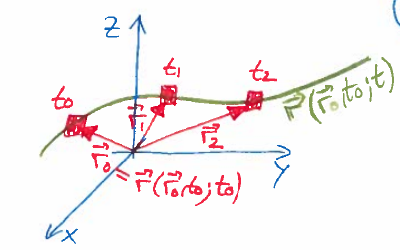
\includegraphics[width=.4\textwidth]{week2/fluid-particle}
    \caption{The path and changing coordinates of a single fluid particle.}
    \label{fig:fluid-particle}
\end{figure}
\begin{align}
\diff{\vec{u}}{t} &= \diff{\vec{u}\left(\vec{r}\left(\vec{r}_0,t_0;t\right),t\right)}{t}\\
&=\diff{\vec{u}(x(\vec{r}_0,t_0;t),y(\vec{r}_0,t_0;t),z(\vec{r}_0,t_0;t))}{t}\\
&=\pdiff{\vec{u}}{x}\diff{x}{t} + \pdiff{\vec{u}}{y}\diff{y}{t} + \pdiff{\vec{u}}{z}\diff{z}{t} + \pdiff{\vec{u}}{t}\diff{t}{t}\\
&= \left(u_x\pdiff{}{x} + u_y\pdiff{}{y} + u_z\pdiff{}{z}\right)\vec{u}+\pdiff{\vec{u}}{t}
\end{align}
\begin{framed}
Short notation for partial derivative:
\begin{equation}
\pdiff{}{x} = \partial_x.
\end{equation}
Here $x$ can be replaced by $y$, $z$ or $t$.

Short notation for velocity:
\begin{equation}
\diff{x}{t} = u_x
\end{equation}
\end{framed}
The terms in parentheses is the dot product between $\vec{u}$ and $\vec{\nabla} = \begin{pmatrix}\partial_x,\ \partial_y,\ \partial_z\end{pmatrix}$,
calculated using the chain rule of differentiation:
\begin{align}
\diff{u(f(t))}{t} &= \pdiff{u}{f}\diff{f}{t}\\
\diff{u(f(t),g(t))}{t} &= \pdiff{u}{f}\diff{f}{t} + \pdiff{u}{g}\diff{g}{t}\\
\diff{u(f(t),g(t),h(t))}{t} &= \pdiff{u}{f}\diff{f}{t} + \pdiff{u}{g}\diff{g}{t} + \pdiff{u}{h}\diff{h}{t}.
\end{align}
This leads to the final expression
\begin{equation}
\diff{\vec{u}}{t} = \pdiff{\vec{u}}{t} + \left(\vec{u}\cdot\vec{\nabla}\right)\vec{u}.
\end{equation}
\begin{framed}
The material derivative is defined as
\begin{equation}
\diff{}{t}\partial_t+\vec{u}\cdot\vec{\nabla}=\frac{D}{Dt}=D_t.
\end{equation}
Whenever we have the time derivative of a field, like $\vec{u}(\vec{r},t)$, then we have to "go with the fluid particle" and use the material derivative.
\end{framed}
We now go back to Newton's second equation:
\begin{equation}
\diff{}{t}(m\vec{u}) = \rho\Delta V\left(\partial_t + \vec{u}\cdot\vec{\nabla}\right)\vec{u} = \vec{F} = \vec{F}_\mathrm{external} + \vec{F}_\mathrm{surrounding}
\end{equation}
The surrounding force can be decomposed into
\begin{equation}
\vec{F}_\mathrm{surrounding} = \vec{F}_\mathrm{pressure} + \vec{F}_\mathrm{friction}
\end{equation}
The surrounding fluid particles push the "sandwiched" fluid particle around; they exert pressure. Mutual friction between neighboring fluid particles due to relative and rotational motion, deformation and compression.

\begin{framed}
\textbf{Example:} The force of gravity is an example of an external force:
\begin{equation}
\vec{F}_\text{external} = \vec{F}_\text{grav} = \underbrace{\rho\Delta V}_m\vec{g}=\rho\vec{g}\Delta V,
\end{equation}
with the gravitational constant defined as
\begin{equation}
\vec{g} = -\begin{pmatrix}
0\\0\\\SI{9.81}{\frac{m}{s}}
\end{pmatrix} = -g\vec{e}_z.
\end{equation}
\end{framed}

\subsection{Pressure force}
\begin{figure}[!h]
    \centering
    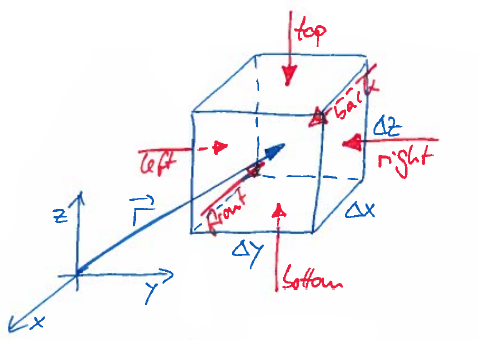
\includegraphics[width=.4\textwidth]{week2/pressure-force}
    \caption{Illustration of the pressure force on each side of a fluid particle.}
    \label{fig:pressure-force}
\end{figure}
\begin{align}
\left(\vec{F}_\mathrm{pressure}\right)_z &= \vec{F}_\mathrm{pressure}^\mathrm{top} + \vec{F}_\mathrm{pressure}^\mathrm{bottom}\\
&= -p\left(x,y,z+\frac{\Delta z}{2}\right)\Delta x \Delta y + p\left(x,y,z-\frac{\Delta z}{2}\right)\Delta x \Delta y \\
\begin{split}&= -\left(p(x,y,z)+\pdiff{p(x,y,z)}{z}\frac{\Delta z}{2}\right)\Delta x \Delta y\\
&\hspace{4.5mm}+ \left(p(x,y,z)+\pdiff{p(x,y,z)}{z}\left(-\frac{\Delta z}{2}\right)\right)\Delta x \Delta y
\end{split}\\
&= -\pdiff{p(x,y,z)}{z} \Delta x \Delta y \Delta z
\end{align}
Using $\Delta x \Delta y \Delta z = \Delta V$ the pressure force density is
\begin{equation}
\vec{f} _\mathrm{pressure} = \frac{\vec{F}_\mathrm{pressure}}{\Delta V} = -\vec{\nabla}p(\vec{r},t)
\end{equation}

\subsection{Friction force}
\begin{figure}[!h]
    \centering
    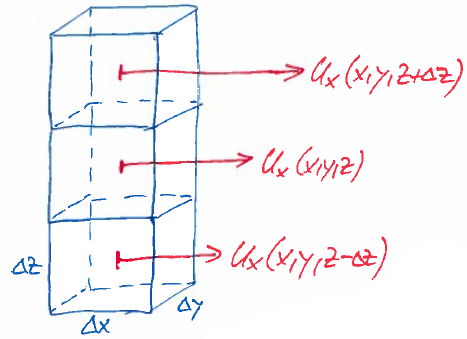
\includegraphics[width=.4\textwidth]{week2/friction-force}
    \caption{Illustration of the friction force on each side of a fluid particle.}
    \label{fig:friction-force}
\end{figure}

We consider the neighboring fluid particles above and below as sketched in \fref{fig:friction-force}.
\begin{equation}
\begin{split}
\left(\vec{F}_\mathrm{friction}^\mathrm{top+bottom}\right)_x &= \frac{\mu}{\Delta z}\Delta x \Delta y \left(u_x(x,y,z+\Delta z)-u_x(x,y,z)\right) \\
&\hspace{4.5mm}+ \frac{\mu}{\Delta z}\Delta x \Delta y \left(u_x(x,y,z-\Delta z)-u_x(x,y,z)\right)
\end{split}
\end{equation}
If $u_x(x,y,z+\Delta z)>u_x(x,y,z)$, then the fluid particle above pulls the sandwiched fluid particle with it.

Taylor series expansion up to second-order terms:
\begin{align}
\begin{split}
\left(\vec{F}_\mathrm{friction}^\mathrm{top+bot}\right)_x &= 
\mu \Delta x\Delta y \left\{\frac{u_x(x,y,z+\Delta z)-u_x(x,y,z)}{\Delta z} +  \frac{u_x(x,y,z-\Delta z)-u_x(x,y,z)}{\Delta z}\right\}\\
&= \frac{\mu\Delta x  \Delta y}{\Delta z}
\left\{u_x(x,y,z)+\pdiff{u_x(x,y,z)}{z}\Delta z + \ppdiff{u_x(x,y,z)}{z}\frac{\Delta z^2}{2} - u_x(x,y,z) \right.\\
&\hspace{4.5mm}  + u_x(x,y,z)+\pdiff{u_x(x,y,z)}{z}(-\Delta z) + \left. \ppdiff{u_x(x,y,z)}{z}\frac{(-\Delta z)^2}{2} - u_x(x,y,z) \right\}
\end{split}\\
&= \mu \Delta x \Delta y \Delta z \ppdiff{u_x(x,y,z)}{z}
\end{align}
Front + back:
\begin{equation}
\left(\vec{F}_\mathrm{friction}^\mathrm{front+back}\right)_x = \mu\Delta V \ppdiff{u_x(x,y,z)}{y}
\end{equation}
Most general expression of the friction force:
\begin{equation}
\frac{\vec{F}_\mathrm{friction}}{\Delta V} = \vec{f}_\mathrm{friction} \left(\pdiff{^2u_i}{x_k\partial x_l}\right) = \vec{f}_\mathrm{friction} (\vec{\nabla},\vec{\nabla},\vec{u})
\end{equation}
The task is to build a vector $\vec{f}$ from a combination of three vectors $\vec{a}=\vec{\nabla}, \vec{b}=\vec{\nabla}, \vec{c}=\vec{u}$, such that
\begin{equation}
\vec{f} = \alpha\left(\vec{a}\cdot\vec{b}\right)\vec{c} + \beta\left(\vec{a}\cdot\vec{c}\right)\vec{b} + \alpha \left(\vec{b}\cdot\vec{c}\right)\vec{a}
\end{equation}
The solution:
\begin{equation}
\vec{f}_\mathrm{friction} = \mu\left(\vec{\nabla}\cdot\vec{\nabla}\right)\vec{u} + \left(\mu_v+\frac{\mu}{3}\right)\vec{\nabla}\left(\vec{\nabla}\cdot\vec{u}\right),
\end{equation}
where $\mu$ is the shear (dynamic) viscosity and $\mu_v$ is the compression (bulk) viscosity.

Navier-Stokes equation:
\begin{equation}
\rho\left(\partial_t+\left(\vec{u}\cdot\vec{\nabla}\right)\right)\vec{u} = \vec{f}_\mathrm{ext}-\vec{\nabla}p + \mu\left(\vec{\nabla}\cdot\vec{\nabla}\right)\vec{u} + \left(\mu_v+\frac{\mu}{3}\right)\vec{\nabla}\left(\vec{\nabla}\cdot\vec{u}\right)
\end{equation}
where
\begin{align}
\vec{u} &= \vec{u}\left(\vec{r},t\right)\\
p &= p\left(\vec{r},t\right)\\
\rho &= \rho\left(\vec{r},t\right)\\
\vec{f}_\mathrm{ext} &= \vec{f}_\mathrm{ext}\left(\vec{r},t\right)
\end{align}


\subsection{Navier-Stokes equation in components}
\begin{align}
\begin{split}\rho
\begin{pmatrix}
\pdiff{u_x}{t} \\ \pdiff{u_y}{t} \\ \pdiff{u_z}{t}
\end{pmatrix} +
\rho
\begin{pmatrix}
\left(u_x\pdiff{}{x}+u_y\pdiff{}{y}+u_z\pdiff{}{z}\right)u_x \\
\left(u_x\pdiff{}{x}+u_y\pdiff{}{y}+u_z\pdiff{}{z}\right)u_y \\
\left(u_x\pdiff{}{x}+u_y\pdiff{}{y}+u_z\pdiff{}{z}\right)u_z
\end{pmatrix} &= 
\begin{pmatrix}
f_x^\mathrm{ext} \\ f_y^\mathrm{ext} \\ f_z^\mathrm{ext}
\end{pmatrix} -
\begin{pmatrix}
\pdiff{p}{x} \\ \pdiff{p}{y} \\ \pdiff{p}{z}
\end{pmatrix} \\
&\hspace{4.5mm}+
\mu
\begin{pmatrix}
\left(\ppdiff{}{x}+\ppdiff{}{y}+\ppdiff{}{z}\right)u_x \\
\left(\ppdiff{}{x}+\ppdiff{}{y}+\ppdiff{}{z}\right)u_y \\
\left(\ppdiff{}{x}+\ppdiff{}{y}+\ppdiff{}{z}\right)u_z
\end{pmatrix} \\
&\hspace{4.5mm}+
\left(\mu_v + \frac{\mu}{3}\right)
\begin{pmatrix}
\pdiff{}{x}\left(\pdiff{u_x}{x}+\pdiff{u_y}{y}+\pdiff{u_z}{z}\right) \\
\pdiff{}{y}\left(\pdiff{u_x}{x}+\pdiff{u_y}{y}+\pdiff{u_z}{z}\right) \\
\pdiff{}{z}\left(\pdiff{u_x}{x}+\pdiff{u_y}{y}+\pdiff{u_z}{z}\right)
\end{pmatrix}
\end{split}
\end{align}

\begin{framed}
\textbf{Remark:} There are only a few exact analytical solutions; many approximate analytical solutions (guided by intuition). Computational fluid dynamics can give us "exact" numerical solutions for approximations to the Navier-Stokes equation.
\end{framed}

We now have three coupled differential equations for five fields: $u_x\left(\vec{r},t\right)$, $u_y\left(\vec{r},t\right)$, $u_z\left(\vec{r},t\right)$, $p\left(\vec{r},t\right)$, and $\rho\left(\vec{r},t\right)$. This means we are missing two equations.


\subsection*{The first missing equation}
From thermodynamics we have an equation of state
\begin{equation}
g(p,\rho)=0.
\end{equation}
For an incompressible flow, the equaiton of state is simply
\begin{equation}
\rho = \mathrm{constant}.
\end{equation}
For a compressible flow, the equation of state can be found with the law of ideal gases:
\begin{equation}
pV=NkT,
\end{equation}
from which we get
\begin{align}
\rho &= \frac{N}{V} = \frac{1}{kT}p\\
\frac{p}{\rho} &= kT = \mathrm{constant}.
\end{align}
This only holds if the temperature is constant.


\subsection*{The second missing equation}
Equation of continuity, local mass conservation.

\begin{figure}[!h]
    \centering
    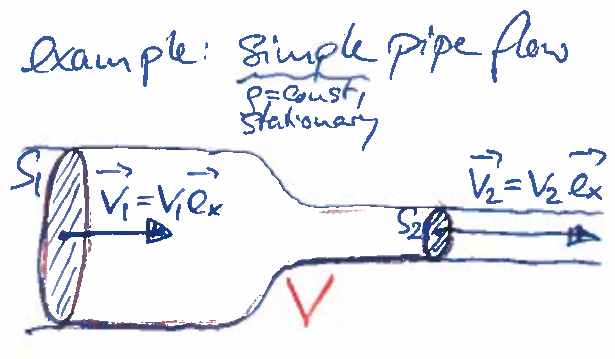
\includegraphics[width=.4\textwidth]{week2/pipe-flow}
    \caption{A simple pipe flow to illustrate mass conservation.}
    \label{fig:pipe-flow}
\end{figure}

\begin{framed}
\textbf{Example:} Simple pipe flow. See \fref{fig:pipe-flow}.
\begin{align}
M_\mathrm{in} &= \rho S_1v_1\Delta t \\
M_\mathrm{out} &= \rho S_2v_2\Delta t
\end{align}
Mass conservation:
\begin{align}
M_\mathrm{in} &= M_\mathrm{out}\\
\leadsto
v_1S_1 &= v_2S_2
\end{align}
This is Leonardo's law.
\end{framed}
Local mass conservation in a small volume element:
\begin{figure}[!h]
    \centering
    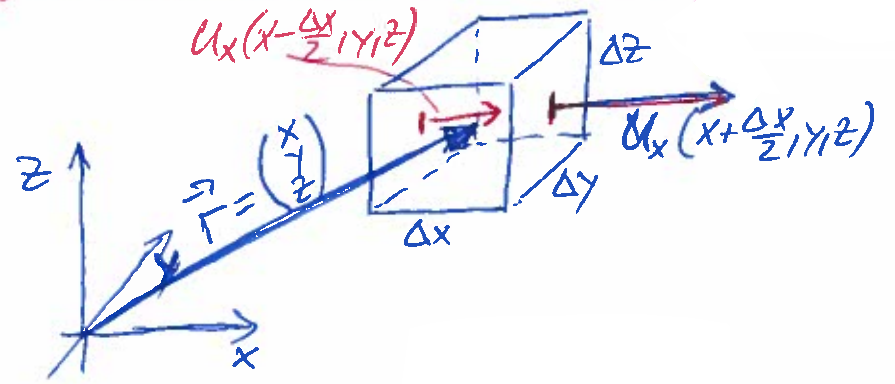
\includegraphics[width=.5\textwidth]{week2/mass-conservation}
    \caption{Local mass conservation in a small volume element.}
    \label{fig:mass-conservation}
\end{figure}

Mass flux through surface of volume $\Delta V = \Delta x \Delta y \Delta z$ in $x$-direction:
\begin{align}
\begin{split}
\diff{M_x^S}{t} &= \rho \left(x+\frac{\Delta x}{2},y,z,t\right)u_x\left(x+\frac{\Delta x}{2},y,z,t\right)\Delta y \Delta z\\
&\hspace{4.5mm} - \rho \left(x-\frac{\Delta x}{2},y,z\right)u_x\left(x-\frac{\Delta x}{2},y,z\right)\Delta y \Delta z
\\
&=\left(\rho(x,y,z)+\pdiff{\rho(x,y,z)}{x}\frac{\Delta x}{2}\right)\left(u_x(x,y,z)+\pdiff{u_x(x,y,z)}{x}\frac{\Delta x}{2}\right) \Delta y \Delta z \\
&\hspace{4.5mm} - \left[\rho(x,y,z)+\pdiff{\rho(x,y,z)}{x}\left(-\frac{\Delta x}{2}\right)\right]\left[u_x(x,y,z)+\pdiff{u_x(x,y,z)}{x}\left(-\frac{\Delta x}{2}\right)\right] \Delta y \Delta z
\\
&=\pdiff{\rho(x,y,z)}{x}u_x(x,y,z)\Delta x \Delta y \Delta z  + \rho(x,y,z)\pdiff{u_x(x,y,z)}{x}\Delta x \Delta y \Delta z\\
&=\pdiff{\left(\rho(x,y,z,t)u_x(x,y,z,t)\right)}{x}\Delta V
\end{split}
\end{align}
Mass flux in $y$ and $z$-direction:
\begin{align}
\diff{M_y^S}{t} &= \pdiff{(\rho(x,y,z)u_y(x,y,z))}{y}\Delta V\\
\diff{M_z^S}{t} &= \pdiff{(\rho(x,y,z)u_z(x,y,z))}{z}\Delta V
\end{align}
Sum of mass fluxes through volume in all directions:
\begin{align}
\diff{M^S}{t} &= \diff{M_x^S}{t} + \diff{M_y^S}{t} + \diff{M_z^S}{t} \\
&= \pdiff{(\rho u_x)}{x}\Delta V + \pdiff{(\rho u_y)}{y}\Delta V + \pdiff{(\rho u_z)}{z}\Delta V\\
&=
\begin{pmatrix}
\pdiff{}{x} \\ \pdiff{}{y} \\ \pdiff{}{z}
\end{pmatrix}
\begin{pmatrix}
\rho u_x \\ \rho u_y \\ \rho u_z
\end{pmatrix}
\Delta V \\
&= \vec{\nabla}\cdot\left(\rho(x,y,z)\vec{u}(x,y,z)\right)\Delta V
\end{align}
Increase of mass within fixed volume $\Delta V$:
\begin{equation}
\pdiff{M^V}{t} = \pdiff{(\rho(\vec{r},t)\Delta V)}{t} = \pdiff{\rho(\vec{r},t)}{t}\Delta V
\end{equation}
Local mass conservation
\begin{equation}
\diff{M^V}{t} = -\diff{M^S}{t}
\end{equation}
If mass within the volume increases, then less has to flow out of the surface than to flow in
\begin{equation}
\pdiff{\rho(\vec{r},t)}{t}+\vec{\nabla}\cdot\left(\rho(\vec{r},t)\vec{u}(\vec{r},t)\right)=0
\end{equation}
This is the equation of continuity.


\subsection{Summary}
Navier-Stokes equation:
\begin{equation}\label{eq:navier-stokes}
\rho\left(\pdiff{}{t}+\left(\vec{u}\cdot\vec{\nabla}\right)\right)\vec{u} = \vec{f} _\mathrm{ext}-\vec{\nabla}p+\mu\left(\vec{\nabla}\cdot\vec{\nabla}\right)\vec{u} + \left(\mu_v + \frac{\mu}{3}\right)\vec{\nabla}\left(\vec{\nabla}\cdot\vec{u}\right)
\end{equation}
\begin{align}
\vec{u} &= \vec{u}(\vec{r},t) = \vec{u}(x,y,z,t) \\
\rho &= \rho(\vec{r},t)\\
p &= p(\vec{r},t)
\end{align}
Equation of continuity:
\begin{equation}
\pdiff{\rho}{t}+\vec{\nabla}\cdot(\rho\vec{u})=0
\end{equation}
Equation of state:
\begin{equation}
g(p,\rho;T)=0
\end{equation}
Heat equation (if the temperature also becomes a field $T(\vec{r},t)$):
\begin{equation}
\left(\pdiff{}{t}+\left(\vec{u}\cdot\vec{\nabla}\right)\right)T(\vec{r},r) = \kappa\left(\vec{\nabla}\cdot\vec{\nabla}\right)T(\vec{r},t),
\end{equation}
where $\kappa$ is the thermal diffusion.
